\documentclass{beamer}

% Theme
\usetheme{Madrid}
\usecolortheme{default}

% Packages
\usepackage{amsmath}
\usepackage{amssymb}
\usepackage{tikz}

% Title Information
\title{Mathematics for Computing}
\subtitle{Assignment 1}
\author{Diya Radhakrishnan}
\institute{
M.Tech in Computer Science and Engineering\\
Specialization in Data Science and Artificial Intelligence\\[0.3cm]
\small Department of Computer Science, CUSAT
}
\date{\today}

\begin{document}

%-------------------------------------------------
% Title
%-------------------------------------------------
\begin{frame}
\titlepage
\end{frame}

%-------------------------------------------------
\begin{frame}{Sets}
\begin{block}{Set}
    A Set is a well-defined, unordered collection of disticnt elements
\end{block}
\begin{block}{Cardinality of a Set}
The number of elements in a set.
\end{block}

\textbf{Example:}

A data scientist chooses the following machine learning algorithms.

\begin{gather*}
A=\{\text{Linear Regression},\text{Decision Tree},
\text{Random Forest},\text{SVM},\text{XGBoost}\}\\
|A|=5
\end{gather*}

\end{frame}

%-------------------------------------------------
\begin{frame}{Types of Sets}

\begin{block}{Finite Set}
A set with a limited number of elements.
\end{block}

\textbf{Example:}

A sentiment analysis dataset has only three labels.

\begin{gather*}
L=\{\text{Positive},\text{Neutral},\text{Negative}\}
\end{gather*}

\end{frame}

%-------------------------------------------------
\begin{frame}{Types of Sets}

\begin{block}{Infinite Set}
A set with unlimited elements.
\end{block}

\textbf{Example:}

A neural network can receive infinitely many real-valued inputs.

\begin{gather*}
X=\{x \mid x\in[0,1]\}
\end{gather*}

\end{frame}

%-------------------------------------------------
\begin{frame}{Types of Sets}

\begin{block}{Null (Empty) Set}
A set with no elements.
\end{block}

\textbf{Example:}

After filtering a dataset for patients older than 200 years, no records remain.

\begin{gather*}
P=\{x\mid x>200\}=\varnothing
\end{gather*}

\end{frame}

%-------------------------------------------------
\begin{frame}{Types of Sets}

\begin{block}{Equal Sets}
Two sets containing exactly the same elements.
\end{block}

\textbf{Example:}

Two ML engineers list identical preprocessing steps.

\begin{gather*}
A=\{\text{Scaling},\text{Imputation},
\text{One-Hot Encoding}\}\\
B=\{\text{One-Hot Encoding},
\text{Scaling},
\text{Imputation}\}\\
A=B
\end{gather*}

\end{frame}

%-------------------------------------------------
\begin{frame}{Types of Sets}

\begin{block}{Equivalent Sets}
Two sets having the same number of elements.
\end{block}

\textbf{Example:}

Three ML models and three deep learning frameworks.

\begin{gather*}
A=\{\text{SVM},
\text{Decision Tree},
\text{Random Forest}\}\\
B=\{\text{TensorFlow},
\text{PyTorch},
\text{Keras}\}\\
|A|=|B|=3
\end{gather*}

\end{frame}

%-------------------------------------------------
\begin{frame}{Types of Sets}

\begin{block}{Subset}
Every element of one set belongs to another set.
\end{block}

\textbf{Example:}

Here set A consists of the Deep Learning models and set B consists of the \\
Machine learning models\\
Deep learning models are a subset of machine learning algorithms.

\begin{gather*}
A=\{\text{CNN},
\text{RNN},
\text{Transformer}\}\\
B=\{\text{CNN},
\text{RNN},
\text{Transformer},
\text{SVM},
\text{Decision Tree}\}\\
A\subseteq B
\end{gather*}

\end{frame}

%-------------------------------------------------
\begin{frame}{Types of Sets}

\begin{block}{Superset}
A set containing all elements of another set.
\end{block}

\textbf{Example:}

Here set A consists of the Deep Learning models and set B consists of the \\
Machine learning models\\
Machine learning algorithms include all deep learning models.
\begin{gather*}
A=\{\text{CNN},
\text{RNN},
\text{Transformer}\}\\
B=\{\text{CNN},
\text{RNN},
\text{Transformer},
\text{SVM},
\text{Decision Tree}\}\\
\end{gather*}
\begin{gather*}
B\supseteq A
\end{gather*}

\end{frame}

%-------------------------------------------------
\begin{frame}{Types of Sets}

\begin{block}{Universal Set}
A set containing every element under consideration.
\end{block}

\textbf{Example:}

All AI algorithms studied in the course.

\begin{gather*}
U=\{
\text{Linear Regression},
\text{Decision Tree},
\text{Random Forest},
\text{SVM},
\text{CNN},\\
\text{RNN},
\text{Transformer}
\}
\end{gather*}

\end{frame}

%-------------------------------------------------
\begin{frame}{Types of Sets}

\begin{block}{Power Set}
The set of all possible subsets.
\end{block}

\textbf{Example:}

Feature selection using Age and Income.

\begin{gather*}
A=\{\text{Age},\text{Income}\}\\
\mathcal{P}(A)=
\{
\varnothing,
\{\text{Age}\},
\{\text{Income}\},
\{\text{Age},\text{Income}\}
\}
\end{gather*}

\end{frame}

%-------------------------------------------------
\begin{frame}{Types of Sets}

\begin{block}{Singleton Set}
A set containing exactly one element.
\end{block}

\textbf{Example:}

Hyperparameter tuning selects only Adam.

\begin{gather*}
O=\{\text{Adam}\}
\end{gather*}

\end{frame}

%-------------------------------------------------
\begin{frame}{Types of Sets}

\begin{block}{Countable Set}
A set whose elements can be counted one by one.
\end{block}

\textbf{Example:}

Datasets stored with unique IDs.

\begin{gather*}
D=\{D_1,D_2,D_3,\ldots\}
\end{gather*}

\end{frame}

%-------------------------------------------------
\begin{frame}{Operations on Sets}
\begin{block}{Union}
The union of two sets contains all elements that belong to either set or both.
\end{block}
\vspace{0.05cm}
\[
A\cup B=\{x\mid x\in A \text{ or } x\in B\}
\]
\textbf{Example:}

Let\vspace{0.05cm}\[
A=\{\text{CNN},\text{RNN}\},\qquad
B=\{\text{RNN},\text{Transformer}\}
\]

Then,\vspace{0.05cm}\[
A\cup B=
\{\text{CNN},\text{RNN},\text{Transformer}\}
\]

\begin{center}
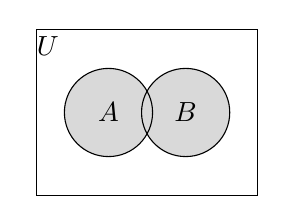
\begin{tikzpicture}[scale=0.7]
\draw (-2,-1.5) rectangle (2,1.5);
\fill[gray!30] (-0.7,0) circle(0.8);
\fill[gray!30] (0.7,0) circle(0.8);
\draw (-0.7,0) circle(0.8);
\draw (0.7,0) circle(0.8);
\node at (-0.7,0) {$A$};
\node at (0.7,0) {$B$};
\node at (-1.8,1.2) {$U$};
\end{tikzpicture}
\end{center}
    
\end{frame}
\begin{frame}{Operations on Sets}

\begin{block}{Intersection}
The intersection of two sets contains the common elements.
\end{block}
\[
A\cap B=\{x\mid x\in A \text{ and } x\in B\}
\]

\textbf{Example:}

\[
A=\{\text{CNN},\text{RNN}\},
\quad
B=\{\text{RNN},\text{Transformer}\}
\]

\[
A\cap B=\{\text{RNN}\}
\]
\begin{center}
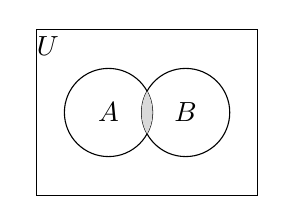
\begin{tikzpicture}[scale=0.7]
\draw (-2,-1.5) rectangle (2,1.5);
\draw (-0.7,0) circle(0.8);
\draw (0.7,0) circle(0.8);
\begin{scope}
\clip (-0.7,0) circle(0.8);
\fill[gray!30] (0.7,0) circle(0.8);
\end{scope}
\node at (-0.7,0) {$A$};
\node at (0.7,0) {$B$};
\node at (-1.8,1.2) {$U$};
\end{tikzpicture}
\end{center}
\end{frame}

\begin{frame}{Operations on Sets}
\begin{block}{Difference of Sets}
The difference of sets contains elements of $A$ that are not in $B$.
\end{block}
\[
A-B=\{x\mid x\in A,\ x\notin B\}
\]

\textbf{Example:}

\[
A=\{\text{CNN},\text{RNN}\},
\quad
B=\{\text{RNN},\text{Transformer}\}
\]

\[
A-B=\{\text{CNN}\}
\]

\end{frame}

\begin{frame}{Operations on Sets}
\begin{block}{Set Difference}
The set difference $B-A$ contains elements of $B$ that are not in $A$.
\end{block}
\[
B-A=\{x\mid x\in B,\ x\notin A\}
\]

\textbf{Example:}

\[
B-A=\{\text{Transformer}\}
\]

\end{frame}

\begin{frame}{Operations on Sets}
\begin{block}{Symmetric Difference}
The symmetric difference contains elements that belong to either set but not both.
\end{block}
\[
A\triangle B=(A-B)\cup(B-A)
\]

\textbf{Example:}

\[
A=\{\text{CNN},\text{RNN}\}
\]

\[
B=\{\text{RNN},\text{Transformer}\}
\]

\[
A\triangle B=
\{\text{CNN},\text{Transformer}\}
\]
\end{frame}

\begin{frame}{Operations on Sets}
\begin{block}{Complement}

The complement of $A$ contains all elements of the universal set that are not in $A$.
\end{block}
\[
A'=U-A
\]

\textbf{Example:}

\[
U=\{\text{CNN},\text{RNN},\text{Transformer}\}
\]

\[
A=\{\text{CNN},\text{RNN}\}
\]

\[
A'=\{\text{Transformer}\}
\]

\end{frame}

\begin{frame}{Operations on Sets}
\begin{block}{Cartesian Product}
The Cartesian product of two sets is the set of all ordered pairs.
\end{block}
\[
A\times B=\{(a,b)\mid a\in A,\ b\in B\}
\]

\textbf{Example:}

Let

\[
A=\{\text{Image},\text{Text}\}
\]

\[
B=\{\text{CNN},\text{Transformer}\}
\]

Then,

\[
A\times B=
\{
(\text{Image},\text{CNN}),
(\text{Image},\text{Transformer}),
(\text{Text},\text{CNN}),
(\text{Text},\text{Transformer})
\}
\]

\end{frame}
%slide 14
\begin{frame}{Examples of Sets in Set Builder form}
    \textbf{1.Squares of first 10 natural numbers}
    \begin{gather*}
        S=\{n^2 \mid n\in\mathbb{N},\ 1\le n\le 10\}
    \end{gather*}
    
    \vspace{0.5cm}
    
    \textbf{2. Set of even numbers in range of 1 to 10}
    \begin{gather*}
        E=\{x\in\mathbb{N}\mid 1\le x\le 10,\; x\text{ is even}\}
    \end{gather*}
\end{frame}


%slide 15
\begin{frame}{Examples of Sets in Set Builder form}
    \textbf{3.Set of prime numbers in less than 20}
    \begin{gather*}
        P=\{x\in\mathbb{N}\mid x<20,\; x\text{ is prime}\}
    \end{gather*}
    
    \vspace{0.5cm}
    
    \textbf{4. Set of all integers between -10 and 10}
    \begin{gather*}
        I=\{x\in\mathbb{Z}\mid -10\le x\le 10\}
    \end{gather*}
\end{frame}

%slide 16
\begin{frame}{Examples of Sets in Set Builder form}
    \textbf{5.Set of all natural numbers which are multiples of 3 but not 7}
    \begin{gather*}
        A=\{x\in\mathbb{N}\mid 3\mid x,\; 7\nmid x\}
    \end{gather*}
    
    \vspace{0.5cm}
    
    \textbf{6.K=\{5,9,7,13,17,....\}}
    \begin{gather*}
        K=\{4n+1\mid n\in\mathbb{N}\}
    \end{gather*}
\end{frame}


%slide 17
\begin{frame}{Examples of Sets in Set Builder form}
    \textbf{7.Set of all natural numbers leaves 2 as remainder when divided by 6}
    \begin{gather*}
        A=\{x\in\mathbb{N}\mid x=6n+2,\; n\in\mathbb{N}_0\}
    \end{gather*}
    
    \vspace{0.5cm}
    
    \textbf{8.A=\{7,14,21,28,...\}}
    \begin{gather*}
        A=\{7n\mid n\in\mathbb{N}\}
    \end{gather*}
\end{frame}


%slide 17
\begin{frame}{Examples of Sets in Set Builder form}
    \textbf{9.Set of factors of 26}
    \begin{gather*}
        F=\{x\in\mathbb{N}\mid x\mid 26\}
    \end{gather*}
    
    \vspace{0.5cm}
    
    \textbf{10.S=\{(4,2),(4,3),(5,2),(8,5),(3,2),(6,4)\}}
    \begin{gather*}
        S=\{(x,y)\mid x,y\in\mathbb{N},\; x>y\}
    \end{gather*}
\end{frame}
% slide 18
\begin{frame}{Inclusion-Exclusion Principle}

\begin{block}
    
{The Inclusion-Exclusion Principle is used to find the number of distinct elements in overlapping sets by adding the sizes of the sets and subtracting their common elements to avoid double counting.}
\end{block}
For two sets,

\[
|A \cup B| = |A| + |B| - |A \cap B|
\]

\texbf Example:

Let
\begin{itemize}
    \item $A$ = Users interested in AI ($|A|=120$)
    \item $B$ = Users interested in Data Science ($|B|=100$)
    \item $|A \cap B|=30$
\end{itemize}

Then,

\[
|A \cup B|
=120+100-30
=190
\]

Hence, \textbf{190 unique users} are interested in AI or Data Science.
\end{frame}

\begin{frame}{General Form of Inclusion-Exclusion Principle}


\vspace{0.3cm}

\textbf{For Two Sets:}

\[
|A \cup B| = |A| + |B| - |A \cap B|
\]

\vspace{0.3cm}

\textbf{For Three Sets}

\[
|A \cup B \cup C|
=
|A|+|B|+|C|
-
|A\cap B|
-
|A\cap C|
-
|B\cap C|
+
|A\cap B\cap C|
\]

\vspace{0.3cm}

\textbf{General Formula (for $n$ sets)}

\[
\left|\bigcup_{i=1}^{n} A_i\right|
=
\sum |A_i|
-
\sum |A_i\cap A_j|
+
\sum |A_i\cap A_j\cap A_k|
-\cdots+
(-1)^{n+1}
\left|\bigcap_{i=1}^{n} A_i\right|
\]

\end{frame}
%slide 21
\begin{frame}{Partially Ordered Sets (Posets)}
\begin{block}{Partially Ordered Sets}

A \textbf{Partially Ordered Set (Poset)} is a set together with a binary relation $\preceq$ that satisfies the following properties for all $a,b,c \in P$:

\begin{itemize}
    \item \textbf{Reflexive:} $a \preceq a$
    \item \textbf{Antisymmetric:} If $a \preceq b$ and $b \preceq a$, then $a=b$
    \item \textbf{Transitive:} If $a \preceq b$ and $b \preceq c$, then $a \preceq c$
\end{itemize}


A poset allows some elements to be incomparable, meaning not every pair of elements must have an order.
\end{block}
\textbf{Example:}
Consider the set of machine learning model complexities,

\[
P=\{\text{Linear Regression},\ \text{Decision Tree},\ \text{Random Forest},\ \text{Deep}\\\hspace{1.7cm}\text{ Neural Network}\}
\]
\end{frame}

%slide22
\begin{frame}{Partially Ordered Sets (Posets)}
Define the relation $\preceq$ as ``\emph{is less complex than or equal to}.'' Then,


\[
\text{Linear Regression}
\preceq
\text{Decision Tree}
\preceq
\text{Random Forest}
\preceq\\\hspace{1.5cm}
\text{Deep Neural Network}
\]

    

This forms a partially ordered set because the relation is reflexive, antisymmetric, and transitive. In practice, such ordering helps compare models based on their complexity, making it useful in AI model selection and Data Science workflows.

\end{frame}

%slide23

\begin{frame}{Example for POSET}
\textbf{Example1: Image Processing}

Let

\[
P=\{\text{Image Acquisition},\ \text{Image Enhancement},\ \text{Image Segmentation}\}
\]

Define the relation $\preceq$ as ``\emph{performed before}.''

\[
\text{Image Acquisition}
\preceq
\text{Image Enhancement}
\]

while \textbf{Image Segmentation} is independent of \textbf{Image Enhancement} for some applications.
Hence, $(P,\preceq)$ is a \textbf{partially ordered set} because not every pair of operations is comparable.
    
\end{frame}

%slide24
\begin{frame}{Examples for POSET}
\textbf{Example2: Deep Learning Models}
Let
\[
P=\{\text{Data Preprocessing},\ \text{Model Training},\ \text{Model Evaluation}\}
\]

Define the relation $\preceq$ as ``\emph{performed before}.''
\vspace{0.3cm}

Then,\\ Data Preprocessing $\preceq$ Model Training and Model Training $\preceq$ Model Evaluation.
\vspace{0.3cm}

Hence, $(P,\preceq)$ is a \textbf{partially ordered set} because the tasks follow a dependency order.
\end{frame}

%slide25
\begin{frame}{Hasse Diagram}

\begin{block}{Hasse Diagram}

A \textbf{Hasse Diagram} is a graphical representation of a partially ordered set (poset). It shows only the \textbf{covering relations} by omitting reflexive, transitive, and redundant edges.
\end{block}
\vspace{0.3cm}

\textbf{Construction Rules}
\begin{itemize}
    \item Place smaller elements below larger elements.
    \item Connect only directly related (covering) elements.
    \item Do not draw arrowheads.
    \item Omit reflexive and transitive relations.
\end{itemize}

\end{frame}

%slide26


\begin{frame}{Hasse Diagram}
\text Let a relation R be defined on a set A\[
A=\{a,b,c\}
\]
    \[
R=\{(a,a),(b,b),(c,c),(d,d),(a,b),(a,c),(b,d),(c,d),(a,d)\}
\]

Removing the reflexive relations,we get 
\[
R=\{(a,b),(a,c),(b,d),(c,d),(a,d)\}
\]
Since,
\[
a \prec b,\quad b \prec d
\;\Rightarrow\;
a \prec d
\]
the transitive relation $(a,d)$ is omitted in the Hasse diagram.
\\Then we get the relation 
\[
R=\{(a,b),(a,c),(b,d),(c,d)\}
\]
\end{frame}
\begin{frame}{Hasse Diagram}

\begin{center}
\begin{tikzpicture}[node distance=1.2cm]
\node (d) {$d$};
\node (b) [below left of=d] {$b$};
\node (c) [below right of=d] {$c$};
\node (a) [below of=b,xshift=0.75cm] {$a$};

\draw (a)--(b);
\draw (a)--(c);
\draw (b)--(d);
\draw (c)--(d);
\end{tikzpicture}
\end{center}

\[
a \prec b,\quad
a \prec c,\quad
b \prec d,\quad
c \prec d
\]

\end{frame}
\end{frame}

%slide27
\begin{frame}{Example of Hasse Diagram}
\textbf{Example: Deep Learning Workflow}\\
Let,
\[
P=\{\text{DataCollection},\ \text{DataPreprocessing},\ \text{ModelTraining},\ \text{ModelEvaluation}\}
\]

with the relation ``performed before''.

\[
\text{DataCollection}
\prec
\text{DataPreprocessing}
\prec
\text{ModelTraining}
\prec
\text{ModelEvaluation}
\]

\begin{center}
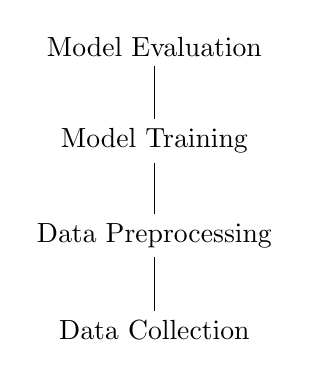
\begin{tikzpicture}[node distance=1.2cm]
\node (A) {Model Evaluation};
\node (B) [below of=A] {Model Training};
\node (C) [below of=B] {Data Preprocessing};
\node (D) [below of=C] {Data Collection};

\draw (D)--(C);
\draw (C)--(B);
\draw (B)--(A);
\end{tikzpicture}
\end{center}

\end{frame}

%slide27
\begin{frame}
    \centering
    \vfill
    {\Huge \textbf{Thank You!}}
    \vfill
\end{frame}





\end{document}